\documentclass[tikz, border=14pt]{standalone}
\usepackage{tikz}
\usepackage{amsmath}
\usepackage{amssymb}
\usetikzlibrary{arrows.meta, positioning, fit, backgrounds, calc}

%% Color palette (shared with controlled_dhgn_lstm_arch.tex / phamiltonian_arch.tex)
\colorlet{Cenc}{blue!65!black}
\colorlet{Cdyn}{violet!75!black}
\colorlet{Copt}{teal!60!black}
\colorlet{Csum}{black!80}

\tikzset{
  lossbox/.style={draw=Cenc, fill=Cenc!8, rounded corners=4pt, thick,
    text width=6.6cm, align=left, minimum height=1.0cm, font=\small},
  dynlossbox/.style={draw=Cdyn, fill=Cdyn!8, rounded corners=4pt, thick,
    text width=6.6cm, align=left, minimum height=1.0cm, font=\small},
  optlossbox/.style={draw=Cenc!70, fill=Cenc!4, rounded corners=4pt, thick,
    dashed, text width=6.6cm, align=left, minimum height=0.9cm, font=\small},
  optdynlossbox/.style={draw=Cdyn!70, fill=Cdyn!4, rounded corners=4pt, thick,
    dashed, text width=6.6cm, align=left, minimum height=0.9cm, font=\small},
  sumbox/.style={draw=Csum, fill=Csum!6, rounded corners=4pt, very thick,
    text width=6.6cm, align=left, minimum height=1.05cm, font=\small},
  arr/.style={-{Stealth[length=6pt, width=4.5pt]}, thick},
  dim/.style={font=\scriptsize, text=black!55},
  weight/.style={font=\scriptsize, text=Copt},
}

\begin{document}
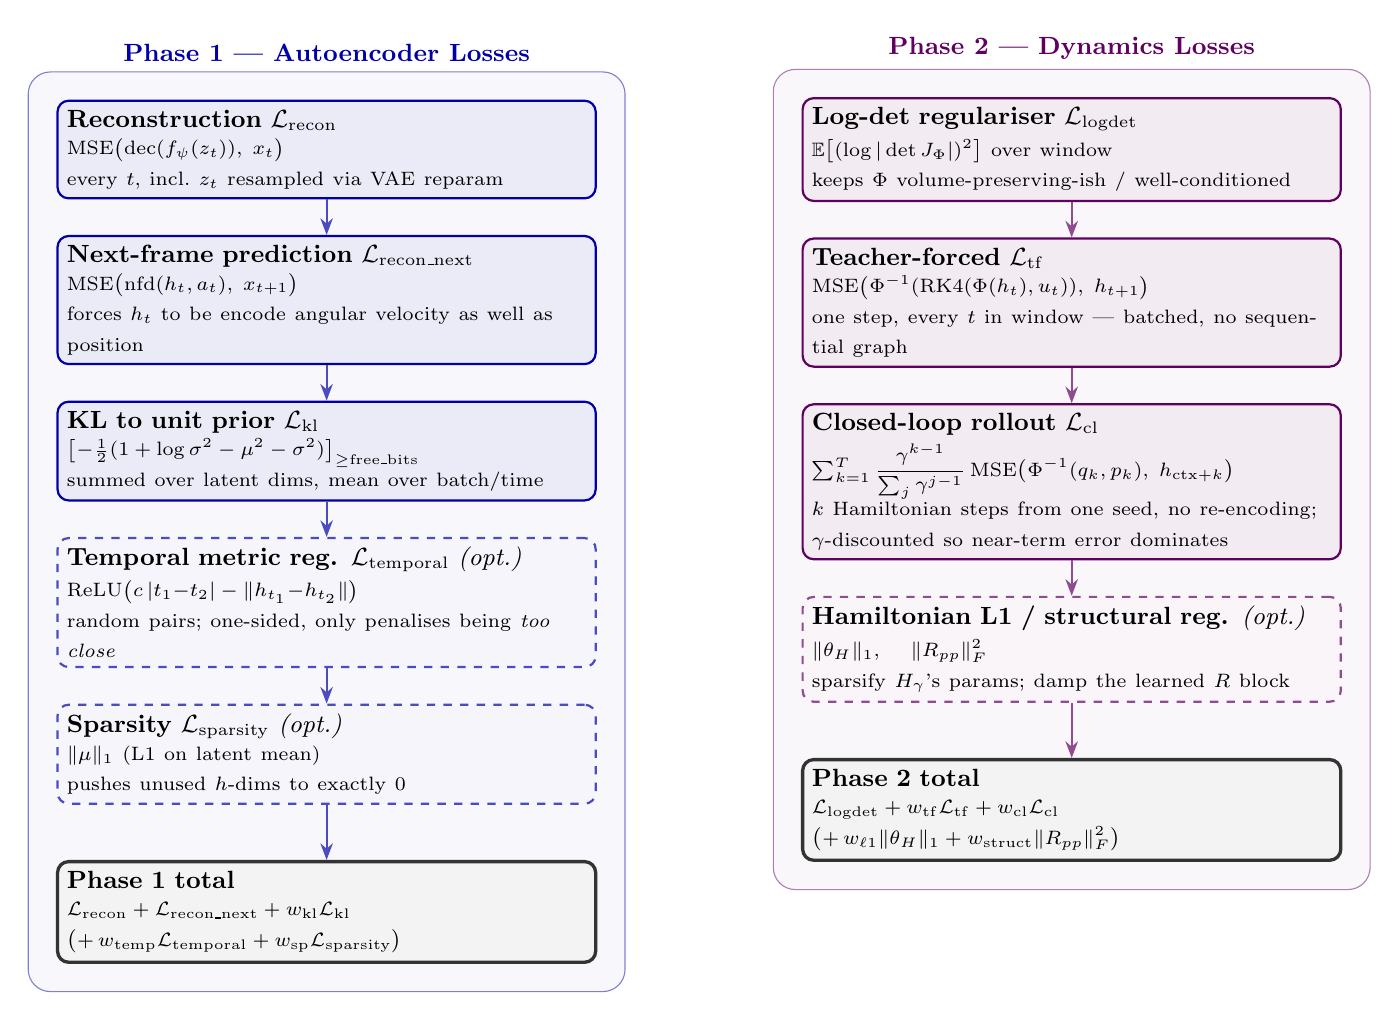
\begin{tikzpicture}[node distance=0.45cm and 2.6cm]

%%==========================================================================
%% LEFT COLUMN — Phase 1: LSTM autoencoder losses
%%==========================================================================

\node[lossbox] (recon)
  {\textbf{Reconstruction} $\mathcal{L}_{\mathrm{recon}}$\\[2pt]
   \scriptsize $\mathrm{MSE}\bigl(\mathrm{dec}(f_\psi(z_t)),\; x_t\bigr)$\\
   \scriptsize every $t$, incl.\ $z_t$ resampled via VAE reparam};

\node[lossbox, below=of recon] (reconnext)
  {\textbf{Next-frame prediction} $\mathcal{L}_{\mathrm{recon\_next}}$\\[2pt]
   \scriptsize $\mathrm{MSE}\bigl(\mathrm{nfd}(h_t, a_t),\; x_{t+1}\bigr)$\\
   \scriptsize forces $h_t$ to be encode angular velocity as well as position};

\node[lossbox, below=of reconnext] (kl)
  {\textbf{KL to unit prior} $\mathcal{L}_{\mathrm{kl}}$\\[2pt]
   \scriptsize $\bigl[-\tfrac{1}{2}(1+\log\sigma^2-\mu^2-\sigma^2)\bigr]_{\ge\text{free\_bits}}$\\
   \scriptsize summed over latent dims, mean over batch/time};

\node[optlossbox, below=of kl] (temporal)
  {\textbf{Temporal metric reg.} $\mathcal{L}_{\mathrm{temporal}}$ \textit{(opt.)}\\[2pt]
   \scriptsize $\mathrm{ReLU}\bigl(c\,|t_1{-}t_2| - \lVert h_{t_1}{-}h_{t_2}\rVert\bigr)$\\
   \scriptsize random pairs; one-sided, only penalises being \emph{too close}};

\node[optlossbox, below=of temporal] (sparsity)
  {\textbf{Sparsity} $\mathcal{L}_{\mathrm{sparsity}}$ \textit{(opt.)}\\[2pt]
   \scriptsize $\lVert \mu \rVert_1$ (L1 on latent mean)\\
   \scriptsize pushes unused $h$-dims to exactly 0};

\node[sumbox, below=0.7cm of sparsity] (sum1)
  {\textbf{Phase 1 total}\\[2pt]
   \scriptsize $\mathcal{L}_{\mathrm{recon}} + \mathcal{L}_{\mathrm{recon\_next}}
     + w_{\mathrm{kl}}\mathcal{L}_{\mathrm{kl}}$\\
   \scriptsize $\bigl(+\,w_{\mathrm{temp}}\mathcal{L}_{\mathrm{temporal}}
     + w_{\mathrm{sp}}\mathcal{L}_{\mathrm{sparsity}}\bigr)$};

%%==========================================================================
%% RIGHT COLUMN — Phase 2: port-Hamiltonian dynamics losses
%%==========================================================================

\node[dynlossbox, right=of recon] (logdet)
  {\textbf{Log-det regulariser} $\mathcal{L}_{\mathrm{logdet}}$\\[2pt]
   \scriptsize $\mathbb{E}\bigl[(\log|\det J_\Phi|)^2\bigr]$ over window\\
   \scriptsize keeps $\Phi$ volume-preserving-ish / well-conditioned};

\node[dynlossbox, below=of logdet] (tf)
  {\textbf{Teacher-forced} $\mathcal{L}_{\mathrm{tf}}$\\[2pt]
   \scriptsize $\mathrm{MSE}\bigl(\Phi^{-1}(\mathrm{RK4}(\Phi(h_t), u_t)),\; h_{t+1}\bigr)$\\
   \scriptsize one step, every $t$ in window — batched, no sequential graph};

\node[dynlossbox, below=of tf] (cl)
  {\textbf{Closed-loop rollout} $\mathcal{L}_{\mathrm{cl}}$\\[2pt]
   \scriptsize $\textstyle\sum_{k=1}^{T} \dfrac{\gamma^{k-1}}{\sum_j \gamma^{j-1}}\,
     \mathrm{MSE}\bigl(\Phi^{-1}(q_k,p_k),\; h_{\mathrm{ctx}+k}\bigr)$\\
   \scriptsize $k$ Hamiltonian steps from one seed, no re-encoding;
   \scriptsize $\gamma$-discounted so near-term error dominates};

\node[optdynlossbox, below=of cl] (l1struct)
  {\textbf{Hamiltonian L1 / structural reg.} \textit{(opt.)}\\[2pt]
   \scriptsize $\lVert \theta_H \rVert_1$, \quad $\lVert R_{pp} \rVert_F^2$\\
   \scriptsize sparsify $H_\gamma$'s params; damp the learned $R$ block};

\node[sumbox, below=0.7cm of l1struct] (sum2)
  {\textbf{Phase 2 total}\\[2pt]
   \scriptsize $\mathcal{L}_{\mathrm{logdet}} + w_{\mathrm{tf}}\mathcal{L}_{\mathrm{tf}}
     + w_{\mathrm{cl}}\mathcal{L}_{\mathrm{cl}}$\\
   \scriptsize $\bigl(+\,w_{\ell 1}\lVert\theta_H\rVert_1
     + w_{\mathrm{struct}}\lVert R_{pp}\rVert_F^2\bigr)$};

%%==========================================================================
%% ARROWS — each term feeds its phase total
%%==========================================================================

\draw[arr, Cenc!70] (recon.south) -- (reconnext.north);
\draw[arr, Cenc!70] (reconnext.south) -- (kl.north);
\draw[arr, Cenc!70] (kl.south) -- (temporal.north);
\draw[arr, Cenc!70] (temporal.south) -- (sparsity.north);
\draw[arr, Cenc!70] (sparsity.south) -- (sum1.north);

\draw[arr, Cdyn!70] (logdet.south) -- (tf.north);
\draw[arr, Cdyn!70] (tf.south) -- (cl.north);
\draw[arr, Cdyn!70] (cl.south) -- (l1struct.north);
\draw[arr, Cdyn!70] (l1struct.south) -- (sum2.north);

%%==========================================================================
%% BACKGROUND GROUPING BOXES
%%==========================================================================
\begin{scope}[on background layer]
  \node[draw=Cenc!50, fill=Cenc!3, rounded corners=8pt, inner sep=10pt,
    fit=(recon)(reconnext)(kl)(temporal)(sparsity)(sum1),
    label={[Cenc, font=\small\bfseries]above:Phase 1 --- Autoencoder Losses}] {};

  \node[draw=Cdyn!50, fill=Cdyn!3, rounded corners=8pt, inner sep=10pt,
    fit=(logdet)(tf)(cl)(l1struct)(sum2),
    label={[Cdyn, font=\small\bfseries]above:Phase 2 --- Dynamics Losses}] {};
\end{scope}

\end{tikzpicture}
\end{document}
